% Comandi personalizzati: modifica qui la grafica senza toccare il codice.
\pagestyle{fancy}
\fancyhf{}
\renewcommand{\headrulewidth}{0.4pt}
\fancyfoot[C]{\small Pag. \thepage\ di \pageref{LastPage}}

% Punteggio a destra della consegna.
\newcommand{\punti}[1]{\hfill\textbf{[#1~pt]}}

% Riga puntinata per lo svolgimento.
\newcommand{\riga}{\noindent\makebox[\linewidth]{\dotfill}\par\vspace{4mm}}

% N righe puntinate (se N = 0 non stampa nulla: il chiamante evita il caso).
\newcommand{\rispostarighe}[1]{\par\vspace{1mm}\foreach \i in {1,...,#1}{\riga}}

% Riquadro per la risposta.
\newcommand{\riquadro}{\par\noindent\framebox[\linewidth]{\rule{0pt}{2.6cm}}\par}

% Griglia quadrettata per grafici e disegni.
\newcommand{\griglia}{\par\noindent
  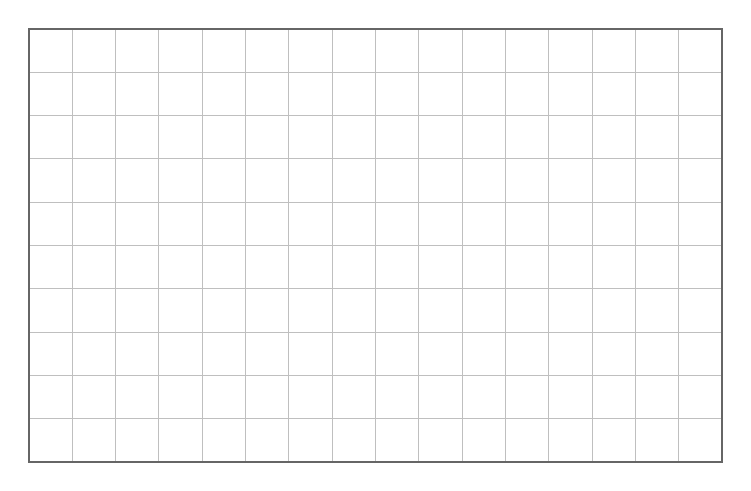
\begin{tikzpicture}[x=0.55cm,y=0.55cm]
    \draw[step=1,lightgray,very thin] (0,0) grid (16,10);
    \draw[black!60,thick] (0,0) rectangle (16,10);
  \end{tikzpicture}\par}

% Piano cartesiano con assi e scala.
\newcommand{\grigliacartesiana}{\par\noindent
  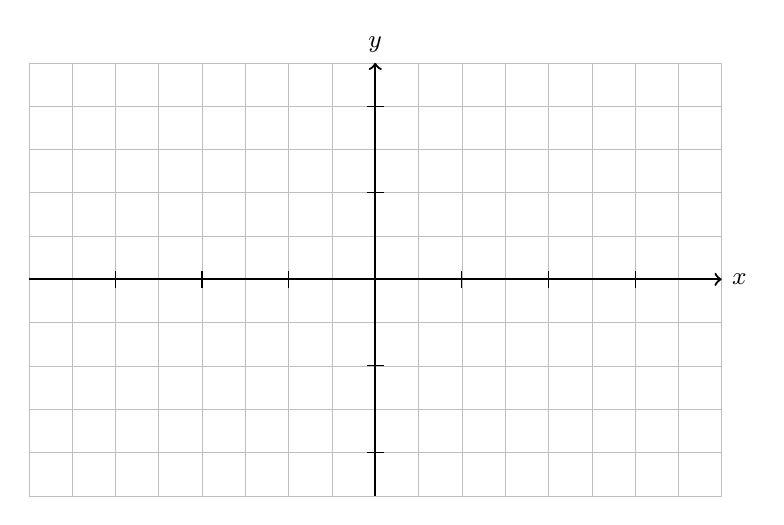
\begin{tikzpicture}[x=0.55cm,y=0.55cm]
    \draw[step=1,lightgray,very thin] (0,0) grid (16,10);
    \draw[->,thick] (0,5) -- (16,5) node[right] {\small $x$};
    \draw[->,thick] (8,0) -- (8,10) node[above] {\small $y$};
    \foreach \x in {2,4,6,10,12,14} \draw (\x,4.8) -- (\x,5.2);
    \foreach \y in {1,3,7,9} \draw (7.8,\y) -- (8.2,\y);
  \end{tikzpicture}\par}

% Intestazione della verifica: istituto, indirizzo, materia, classe, data, tempo, punti, soglia.
\newcommand{\intestazione}[8]{%
  \begin{center}
    {\large\bfseries #1}\\[1mm]
    {\small #2\ --\ #3}\\[3mm]
    {\Large\bfseries #4}\\[3mm]
    \begin{tabular}{@{}p{0.48\textwidth}p{0.48\textwidth}@{}}
      Classe: #5 & Data: #6 \\
      Tempo: #7 & Punteggio: #8 \\
    \end{tabular}
  \end{center}
}

% Titolo di sezione con spazio garantito.
\newcommand{\titolosezione}[1]{\par\needspace{4\baselineskip}\section*{#1}\vspace{-1mm}}

% Blocco soluzione.
\newcommand{\soluzione}[1]{\par\noindent #1\par}

% Casella per gli errori comuni (soluzioni).
\newcommand{\erroricomuni}[1]{%
  \par\smallskip
  \noindent\fcolorbox{black!25}{black!3}{%
    \begin{minipage}{\dimexpr\linewidth-2\fboxsep-2\fboxrule\relax}
      \small\textbf{Errori comuni attesi:} #1
    \end{minipage}}\par\smallskip
}
